\documentclass[titlepage]{article}

\usepackage[utf8]{inputenc}
\usepackage[ngerman]{babel}
\usepackage{graphicx}

\author{Stefanie Gareis}
\title{Das Modell freedom.mdl}
\date{\today}

\begin{document}

\maketitle
\pagenumbering{Roman}
\tableofcontents
\newpage
\pagenumbering{arabic}
\setcounter{page}{1}

\section{Simulink}
Simulink ist ein recht umfangreiches Simulationsprogramm, bei dem ein Modell mit Blöcken aufgebaut wird. Ein großer Vorteil von Simulink ist die Verwendung eine VRML-Welt, mit der man das zu simulierende Objekt auch grafisch darstellen kann.\\
Zusätzlich zu den von Simulink bereitgestellten Blöcken ist es auch möglich Matlab-Funktionen in das Diagramm einzubinden, um Funktionen bereitzustellen die Simulink nicht bietet.

\section{Aufbau des Modells}

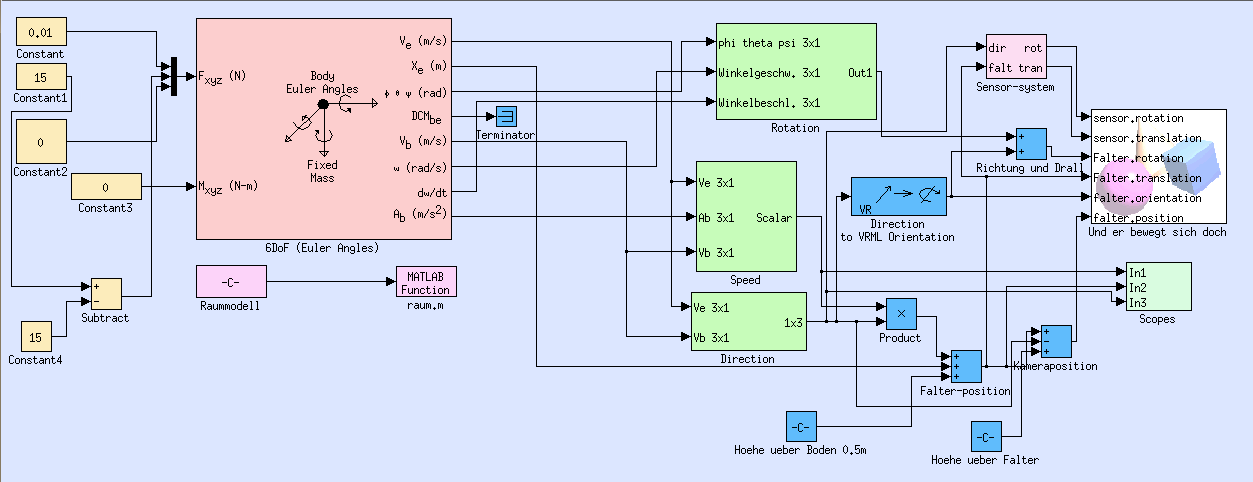
\includegraphics[width=\linewidth]{modell.png}
\\
\\
Das Modell freedom.wrl besitzt vier \glqq Hauptblöcke\grqq \, die die Hauptarbeit der Simulation erledigen. Diese sind 6DoF (Euler Angles), Rotation, Speed und Direction.

\subsection{6 Degrees of Freedom (=6DoF) - Euler Angles}
Dieser Block erledigt alle aeronautischen Berechnungen um aus wenigen Kräften Geschwindigkeit, Flughöhe, und Rotationen zu berechnen. Es gibt acht Ausgänge von denen für dieses Modell nur sieben notwendig sind.\\
$V_{e}$ und $V_{b}$ sind Geschwindigkeiten, einmal im Bezug zur Erde und einmal im Bezug zum Objekt; $A_{b}$ ist die Beschleunigung die das Objekt erfährt und $X_{e}$ ist seine aktuelle Position, aus diesen Daten lässt sich die Bewegung des Falters ermitteln.\\
$\Phi$, $\Theta$ und $\Psi$  sind die drei Eulerschen Winkel, die die Drehung um die Eigene Achse beschreiben, die Geschwindigkeit dieser Drehung wird mit $\omega$ beschreiben, ihre Beschleunigung mit d$\omega$/dt.

\subsection{Rotation}
Der {\em Rotation}--Block ist ein selbst erstelltes Subsystem, welches als Eingangsparameter die Eulerschen Winkel $\Phi$, $\Theta$ und $\Psi$, die Winkelgeschwindigkeit $\omega$ und die Winkelbeschleunigung $\omega$ besitzt.\\
Der Ausgangsvektor enthält die entsprechende Rotationsachse und die Größe des Winkels, um den gedreht wird.

\subsection{Speed}
Das Subsystem {\em Speed} erhält als Eingangsparameter $V_e$, $A_b$ und $B_b$, aus diesen wird dann die Summe gebildet, von dieser der Betrag berechnet und als Skalar wieder ausgegeben, um anschließend weiterverarbeitet zu werden.

\subsection{Direction}
Der Block {\em Direction} berechnet aus den Eingangsvektoren $V_e$ und $V_b$ einen Ausgangsvektor, der die normierte Richtung darstellt, diese Multipliziert mit der Geschwindigkeit ergibt die Ortsveränderung.

\section{Schnittstelle VRML-Simulink}
Die Schnittstelle zwischen VRML und Simulink ist der Block \glqq VR Sink\grqq \ . Mit diesem Block kann man einen VR-Viewer öffnen und dort die entsprechenden Block Parameter ändern. Hier kann man eine Welt auswählen und ihre Knoten verändern, so dass das gewünschte auch sichtbar wird.\\
Die Ausgänge der vorangegangenen Blöcke werden noch ein wenig verrechnet um korrekte Darstellungen zu liefern und landen dann in den Eingängen Falter.rotation, Falter.translation, falter.orientation und falter.position. Die kleingedruckten falter-Felder greifen auf die Kamera zu, die anderen direkt auf den Falter, auf dass er sich bewege und die Welt entdecke.
\end{document}
